\chapter{Minimum Spanning Tree}

Sebuah Spanning Tree merupakan sebuah potongan graph (subgraph) satu arah yang menghubungkan semua vertex menjadi sebuah tree. Sebuah graph dapat memiliki beberapa Spanning Tree sekaligus. Gambar~\ref{fig:spanning-tree-intro} menunjukkan contoh beberapa Spanning Tree dari sebuah graph.

\begin{figure}
    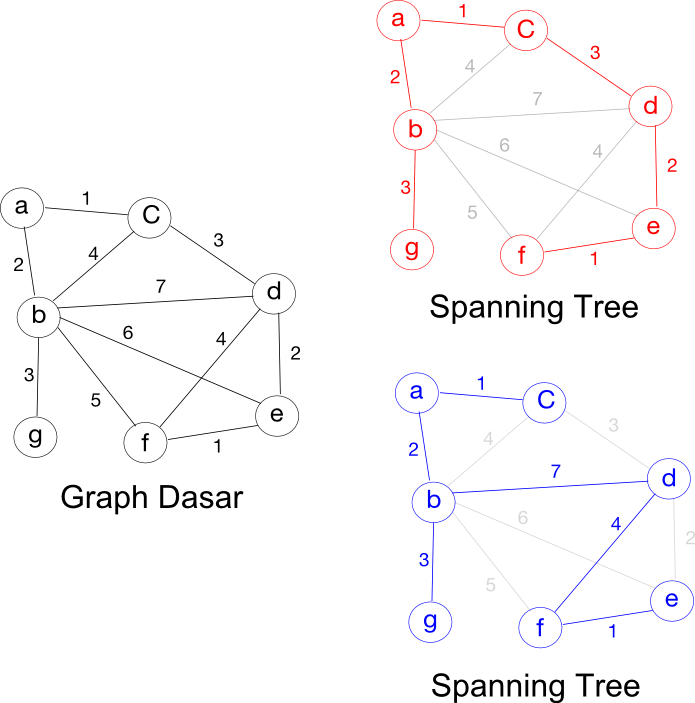
\includegraphics[width=\textwidth,keepaspectratio]{fig/SpanningTreeIntro.png}%
	\caption{Spanning Tree dalam sebuah Graph}%
	\label{fig:spanning-tree-intro}%
\end{figure}

Ketika menggambarkan sebuah Spanning Tree, kita dapat mengalokasikan nilai untuk setiap edge di dalamnya. Total bobot dari keseluruhan edge yang ada di dalam sebuah Spanning Tree kita kenal dengan istilah \textit{weight}. Sebuah Spanning Tree yang memiliki total nilai \textit{weight} terendah kita kenal dengan nama \textbf{Minimum Spanning Tree (MST)}.

MST memiliki banyak aplikasi pada perancangan sistem, terutama untuk sistem-sistem yang berhubungan dengan jaringan. Salah satu contoh pemanfaatan MST yaitu ketika sebuah perusahaan listrik ingin menambahkan jangkauan listrik ke suatu daerah, dengan memasang tiang listrik. Pemasangan tiang listrik pada suatu daerah akan dibatasi oleh berbagai batasan fisik, misalnya perusahaan listrik tidak mungkin memasang tiang listrik di dalam rumah penduduk. Jika kita mengasumsikan pemasangan hanya dilakukan pada sepanjang jalan, kita dapat membangun graph untuk merepresentasikan titik-titik yang dapat menjadi tempat pemasangan tiang listrik. Gambar~\ref{fig:electricity-installation} menggambarkan graph yang mungkin kita bangun untuk pemasangan listrik dalam sebuah kota.

\begin{figure}
    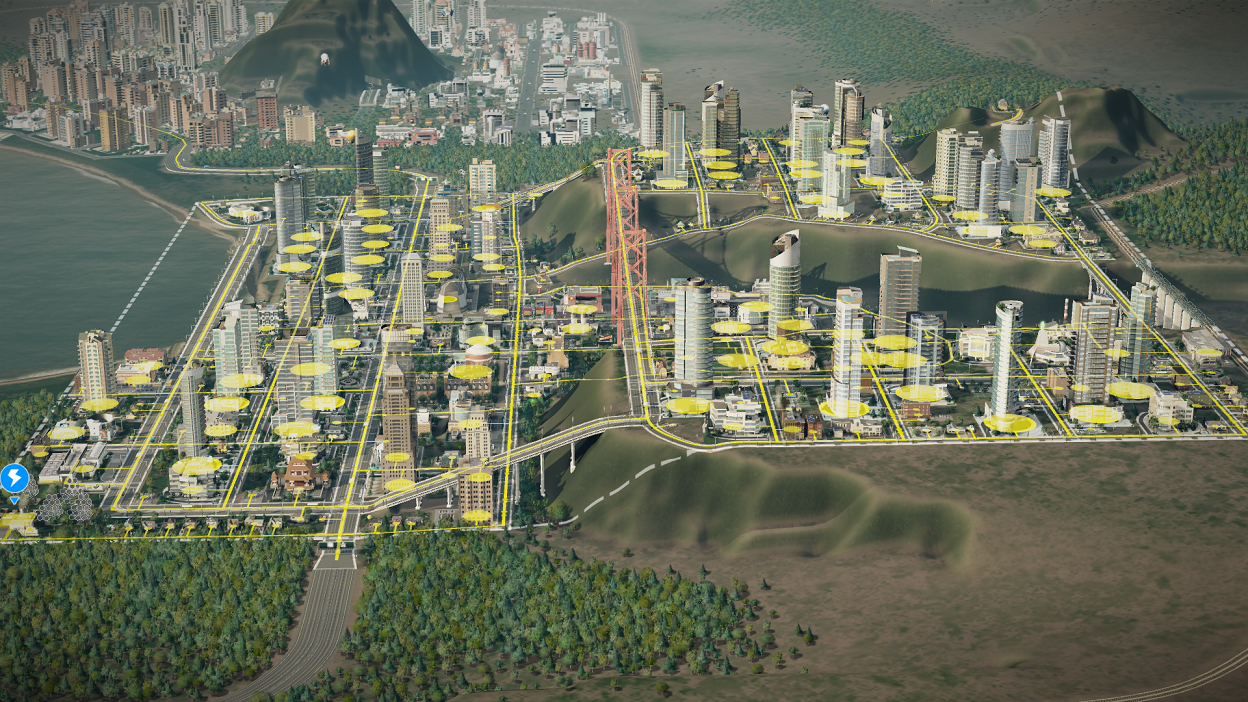
\includegraphics[width=\textwidth,keepaspectratio]{fig/ElectricityInstallation.png}%
	\caption{Jalur Pemasangan Tiang Listrik dalam Graph (Lingkaran Kuning adalah Vertex)}%
	\label{fig:electricity-installation}%
\end{figure}

Ketika sudah memiliki graph untuk jalur pemasangan tiang listrik seperti pada gambar~\ref{fig:electricity-installation}, kita kemudian dapat memberikan bobot kepada masing-masing edge yang ada. Acuan untuk nilai bobot yang digunakan dapat berbeda-beda, tergantung dari tujuan yang ingin dicapai. Contoh dari acuan yang dapat digunakan adalah jarak antar titik. Selain itu, kita juga dapat menggunakan biaya pemasangan sebagai tolak ukur bobot. Pemasangan tiang listrik pada sebuah bukit tentunya akan lebih mahal dan sulit, meskipun mungkin jarak yang ditempuh akan menjadi lebih sedikit.

Setelah memiliki graph pemasangan dan memilih acuan bobot dari edge, kita kemudian dapat mengguankan MST untuk menentukan jalur pemasangan listrik yang paling optimal. Metode pemanfaatan MST yang seperti ini dapat kita terapkan pada berbagai proses lain, seperti pemasangan kabel telepon, segmentasi gambar, dan lain-lain.

\section{Syarat dan Sifat MST}

Berdasarkan kajian singkat yang telah kita bahas pada bagian sebelumnya, terdapat beberapa kesimpulan yang dapat kita tarik. Pertama, sebelum membangun sebuah MST, kita terlebih dahulu harus memiliki dua hal berikut:

\begin{enumerate}
    \item Sebuah Graph satu arah
    \item Bobot dari masing-masing edge di dalam graph
\end{enumerate}

Kedua, sifat-sifat umum yang dimiliki oleh sebuah MST yaitu:

\begin{enumerate}
    \item Sebuah graph dapat memiliki banyak MST
    \item Jika setiap edge yang ada dalam graph memiliki nilai unik, maka hanya akan terdapat satu MST di dalam graph tersebut
    \item Jika bobot dari semua edge selalu bernilai positif, MST yang didapatkan akan selalu merupakan subgraph dengan bobot terkecil yang menghubungkan seluruh vertex
\end{enumerate}

Pembentukan MST dari sebuah graph sendiri merupakan permasalahan optimasi yang dapat kita selesaikan dengan algoritma greedy. Pada bagian berikutnya kita akan membahas dua buah algoritma umum yang digunakan untuk membangun MST, yaitu algoritma Kruskall dan Prim.

\section{Algoritma Kruskall}

\section{Algoritma Prim}
